\documentclass[12pt]{report}
\usepackage{amsthm}
\usepackage{amssymb}
\usepackage{amsmath}
\usepackage{listings}
\usepackage{graphicx}
\usepackage{float}
\usepackage{xcolor}
\usepackage{hyperref}

\hypersetup{
    colorlinks=true,
    linkcolor=black,
    filecolor=magenta,      
    urlcolor=blue,
    pdftitle={Relazione progetto e-commerce},
    pdfpagemode=FullScreen,
}

\setlength{\parindent}{0pt}
\setlength{\parskip}{5pt}

\begin{document}
    \renewcommand{\labelenumii}{\arabic{enumi}.\arabic{enumii}}
    \renewcommand{\labelenumiii}{\arabic{enumi}.\arabic{enumii}.\arabic{enumiii}}
    \renewcommand{\labelenumiv}{\arabic{enumi}.\arabic{enumii}.\arabic{enumiii}.\arabic{enumiv}}

    \title{Relazione progetto e-commerce}
    \author{A. Bandiera (1985878) - I. Radu Barbalata (2002688)\\S. Bianco (1986936) - S. Lazzaroni (1983548)}
    \date{\today}

    \maketitle
    \tableofcontents
    \newpage

    \chapter{Descrizione generale}
    

    Si vuole progettare una piattaforma di e-commerce, nella quale grandi fornitori possono mettere in vendita prodotti per acquirenti privati.

    Un acquirente deve potersi registrare sulla piattaforma attraverso una e-mail, il proprio nome, il proprio cognome ed un recapito telefonico; inoltre, per effettuare ordini ogni acquirente deve indicare almeno un indirizzo per la consegna dei propri acquisti, ed ogni indirizzo è contrassengato da CAP, via, numero civico, città e nazione di appartenenza. Ogni utente deve anche registrare almeno una carta per effettuare gli acquisti, la quale è definita dal proprio codice identificativo. Infine, il sistema deve poter permettere agli acquirenti di cercare i prodotti della piattaforma per nome, ed ogni acquirente deve poter lasciare un feedback ai prodotti da lui acquistati, rappresentato da un punteggio da 1 a 5 stelle.

    Un prodotto è costituito da un codice identificativo, un nome, una descrizione ed il prezzo. Ogni acquirente può ordinare i vari prodotti presenti all'interno della piattaforma, resi disponibili da fornitori; all'interno di un ordine l'acquirente può scegliere la quantità di ogni prodotto che desidera acquistare, anche di vari fornitori. Il costo dell'acquisto è pari al totale dei prezzi dei prodotti ordinati, sommato al costo di spedizione, il quale è costituito da una tariffa fissa imposta dal servizio di e-commerce, indipendente dai prodotti e dai fornitori. Inoltre, è possibile annullare gli ordini effettuati prima che questi vengano spediti all'acquirente. Se l'acquirente è insoddisfatto di alcuni prodotti ricevuti all'interno di un acquisto, il sistema permette di effettuarne il reso gratuitamente.

    Un fornitore, ovvero un'azienda privata, deve potersi registrare inserendo nel sistema la propria ragione sociale. Inoltre, ogni fornitore deve poter registrare, modificare e rifornire i prodotti che desidera mettere in vendita, e può verificare quale siano i prodotti maggiormente venduti in un lasso temporale specificato.

    I trasportatori sono costituiti da aziende private di trasporto merci, che possono registrarsi sulla piattaforma attraverso la propria ragione sociale, ed hanno accesso alla gestione delle spedizioni da loro effettuate; in particolare, si occuperanno di prendere in carico gli ordini a cui non è ancora stato assegnato uno spedizioniere, notificare l'avvenuta consegna di un ordine, l'avvenuto reso o l'eventuale perdita del pacco da consegnare.


    \chapter{Analisi del software}

    \section{User requirements}

    \subsection{Lista dei requisiti}
   
    \begin{enumerate}
        \item Customer
            \begin{enumerate}
                \item Registrazione alla piattaforma
                    \begin{enumerate}
                        \item E-mail
                        \item Nome
                        \item Cognome
                        \item Recapito telefonico
                        \item Indirizzo
                            \begin{enumerate}
                                \item CAP
                                \item Via
                                \item Numero civico
                                \item Città
                                \item Nazione
                            \end{enumerate}
                    \end{enumerate}
                \item Registrazione carte
                    \begin{enumerate}
                        \item Codice identificativo
                    \end{enumerate}
                \item Effettuare ordini di vari prodotti attualmente disponibili
                    \begin{enumerate}
                        \item Quantità per ogni prodotto
                        \item Carta del customer
                        \item Indirizzo di spedizione del customer
                    \end{enumerate}
                \item Cancellare un ordine effettuato
                \item Effettuare resi gratuiti dei propri ordini
                    \begin{enumerate}
                        \item Prodotti e quantità di prodotto da restituire
                    \end{enumerate}
                \item Ricerca prodotti per nome
                \item Recensire prodotti da loro acquistati attraverso punteggio in [1, 5]
            \end{enumerate}
        \item Fornitore
            \begin{enumerate}
                \item Registrazione alla piattaforma
                    \begin{enumerate}
                        \item Ragione sociale
                    \end{enumerate}
                \item Gestione prodotti (registrazione, modifica e rifornimento)
                    \begin{enumerate}
                        \item Codice identificativo
                        \item Nome
                        \item Descrizione
                        \item Prezzo
                    \end{enumerate}
                \item Statistiche prodotti
                    \begin{enumerate}
                        \item Prodotti maggiormente venduti in un dato arco temporale
                    \end{enumerate}
            \end{enumerate}
        \item Trasportatore
            \begin{enumerate}
                \item Registrazione alla piattaforma
                    \begin{enumerate}
                        \item Ragione sociale
                    \end{enumerate}
                \item Gestione spedizioni
                    \begin{enumerate}
                        \item Prendere in carico spedizioni
                        \item Notificare l'avvenuta consegna di ordini
                        \item Notificare l'avvenuto reso di ordini
                        \item Notificare lo smarrimento di un ordine
                    \end{enumerate}
            \end{enumerate}
    \end{enumerate}

    \newpage

    \subsection{Entity-Relationship diagram}
    
    \begin{figure}[H]
        \centering
        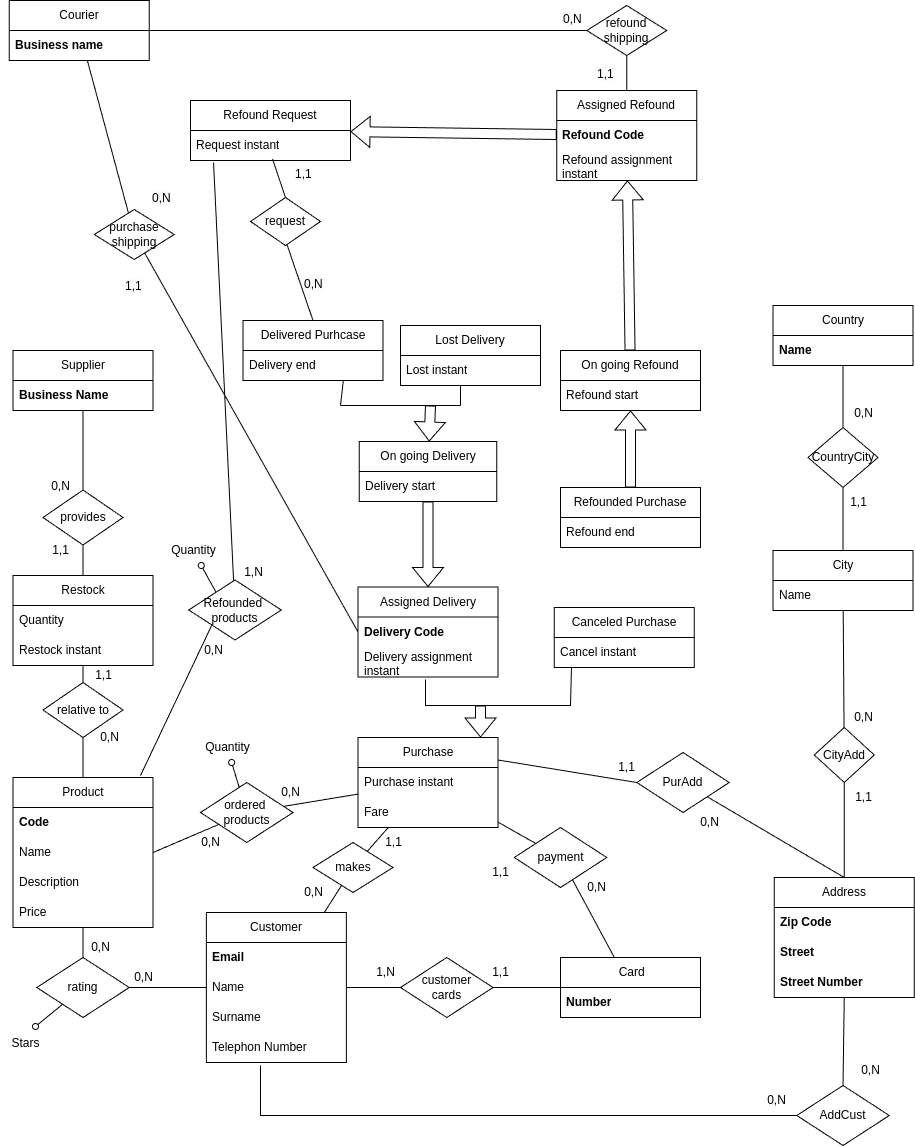
\includegraphics[scale=0.44]{images/ER-Expanded.png}
        
        \label{fig:entity_rel_diagram}
    \end{figure}
    
    \subsection{Use-case diagram}
    
    \begin{figure}[H]
        \centering
        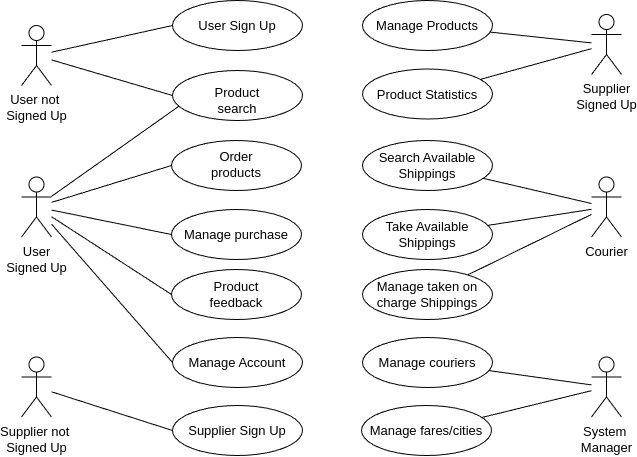
\includegraphics[scale=0.6]{images/Use-cases.png}
        \caption{Diagramma degli use-case}
        \label{fig:use_cases}
    \end{figure}

    \newpage
    
    \section{System requirements}

    \subsection{Requisiti funzionali e non-funzionali}

    \begin{enumerate}
        \item Customer
        \begin{enumerate}
            \item Effettuare acquisti
            \begin{enumerate}
                \item Ogni acquisto deve essere effettuato da un customer, attraverso una delle carte di credito da lui registrate
                \item Ogni acquisto deve essere spedito ad uno degli indirizzi registrati da parte del customer che ha effettuato l'acquisto
                \item Il numero di prodotti che vengono acquistati all'interno di un ordine non deve eccedere le disponibilità dei fornitori registrate all'interno del sistema
                \item I prodotti acquistati all'interno di un ordine possono essere di diversi fornitori
            \end{enumerate}
            \item Cancellare ordini
            \begin{enumerate}
                \item Un ordine può essere cancellato solamente se non è stato ancora preso in carico da nessun corriere
            \end{enumerate}
            \item Effettuare resi
            \begin{enumerate}
                \item Il reso di un ordine può essere effettuato solamente dopo aver ricevuto l'ordine all'indirizzo indicato
                \item Il reso di un ordine può essere effettuato solamente da parte del customer che aveva fatto l'acquisto
                \item La quantità di prodotto della quale un customer vuole effettuarne il reso non deve eccedere la quantità di prodotto presente all'interno dell'ordine originale
            \end{enumerate}
            \item Recensire prodotti
            \begin{enumerate}
                \item Un customer può recensire un prodotto solamente se ha precedentemente effettuato un acquisto che lo conteneva
            \end{enumerate}
        \end{enumerate}
        \item Fornitori
        \begin{enumerate}
            \item Gestione prodotti
            \begin{enumerate}
                \item L'unica caratteristica che è possibile modificare dei prodtotti è la loro descrizione
            \end{enumerate}
            \item Gestione restock
            \begin{enumerate}
                \item Se un fornitore desidera mettere a disposizione nuove scorte di un dato prodotto deve necessariamente registrare una nuova istanza di restock, e non può modificare le istanze già esistenti
            \end{enumerate}
        \end{enumerate}
        \item Trasportatori
        \begin{enumerate}
            \item Gestione spedizioni
            \begin{enumerate}
                \item Le spedizioni che possono essere prese in carico sono quelle di cui nessun altro trasportatore si è ancora fatto carico
            \end{enumerate}
            \item Notificare l'avvenuta consegna di ordini
            \begin{enumerate}
                \item È possibile notificare l'avvenuta consegna di un ordine solamente se il pacco non è andato perduto
            \end{enumerate}
            \item Notificare la perdita di ordini
            \begin{enumerate}
                \item È possibile notificare la perdita di un pacco solamente se questo non è stato ancora consegnato
            \end{enumerate}
        \end{enumerate}

        \item Requisiti non-funzionali
        
        \begin{enumerate}
            \item Il tempo medio di sessione di un client deve essere inferiore a 30 secondi
            \item Il tempo medio di risposta del server ad una richiesta da parte di un client deve essere inferiore a 30 secondi
        \end{enumerate}
    \end{enumerate}

    \newpage
    
    \subsection{Architettura del sistema}
    
    Il sistema viene progettato seguendo un approccio basato sulla separazione delle richieste ricevute dal sistema. In particolare, l'intero sistema viene decentralizzato in tre server: un server accessibile dai \textbf{clienti}, un server accessibile dai \textbf{fornitori} ed un server accessibile dai \textbf{trasportatori}. Ognuno dei tre server è eseguito parallelamente agli altri due e si occupa di gestire e soddisfare solo ed esclusivamente le tipologie di richieste ad esso designate.

    \begin{figure}[H]
        \centering
        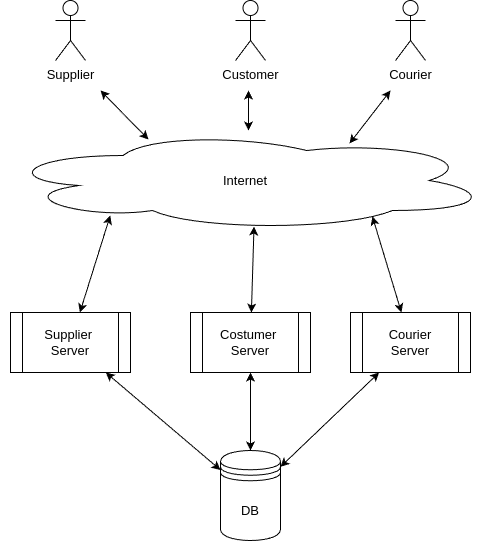
\includegraphics[scale=0.5]{images/System Architecture.png}
        \caption{Architettura fisica del sistema}
        \label{fig:physical_architecture}
    \end{figure}
    
    Ognuno dei tre server viene a sua volta suddiviso in due componenti, un primo modulo denominato \textbf{Server}, addetto alla gestione delle richieste ricevute da e inviate a ognuno degli utenti connessi al sistema, e un secondo modulo denominato \textbf{Handler}, addetto alla gestione dello smistamento delle richieste tra vari processi in esecuzione sul server stesso, inviando ogni richiesta tramite uno stream Redis al processo incaricato. 

    \newpage
    
    Ciascuno di tali processi viene denominato \textbf{Manager}. Ogni Manager è una macchina a stati finiti (vedere sezioni successive) che rimane in attesa di ricevere una richiesta da parte dell'Handler associato, per poi processare tale richiesta interagendo con il database ed infine restituire l'esito all'Handler.
    
    \begin{figure}[H]
        \centering
        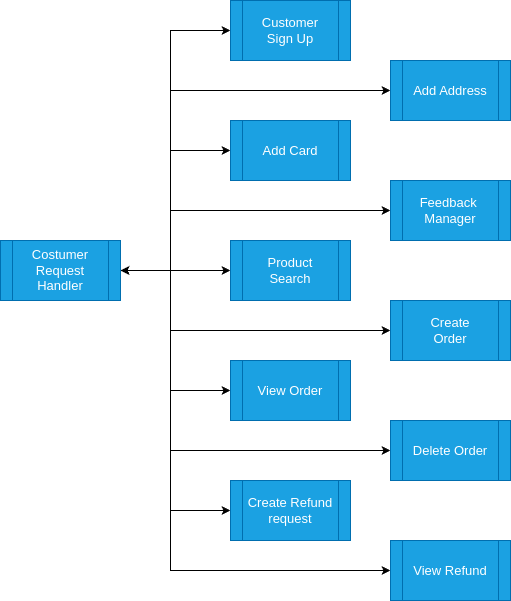
\includegraphics[scale=0.6]{images/System Architecture 1.png}
        \caption{Associazioni tra Customer Handler e i suoi manager}
        \label{fig:Manager_architecture_1}
    \end{figure}
    
    \begin{figure}[H]
        \centering
        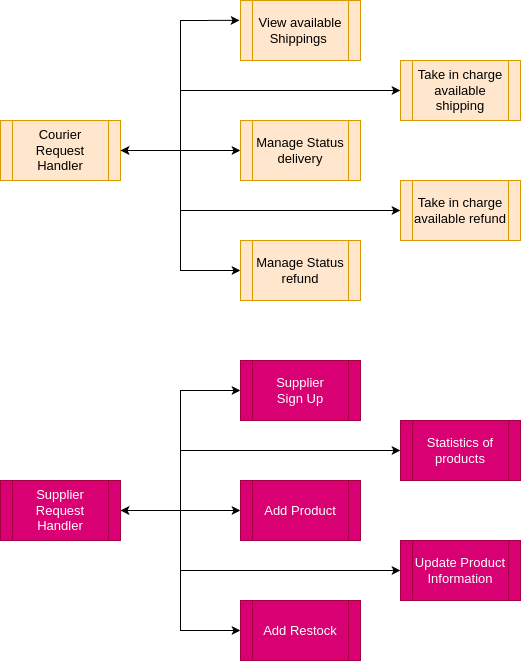
\includegraphics[scale=0.6]{images/System Architecture 2.png}
        \caption{Associazioni tra Courier e Supplier Handler e i loro manager}
        \label{fig:Manager_architecture_2}
    \end{figure}

    \newpage
    
    \subsection{Activity diagram}

    Di seguito viene riportato l'activity diagram relativo all'invio di una richiesta da parte di un client, l'elaborazione di essa e dell'invio della risposta da parte del server. Tale processo risulta comune per tutti i server e i loro Manager, indipendentemente dal tipo di richiesta effettuata dal client. Inoltre, è necessario specificare che, nello scenario descritto, il client abbia già precedentemente stabilito la connessione con il server e che il Manager incaricato sia già attivo e pronto a ricevere e processare una richiesta.
    
    \begin{figure}[H]
        \centering
        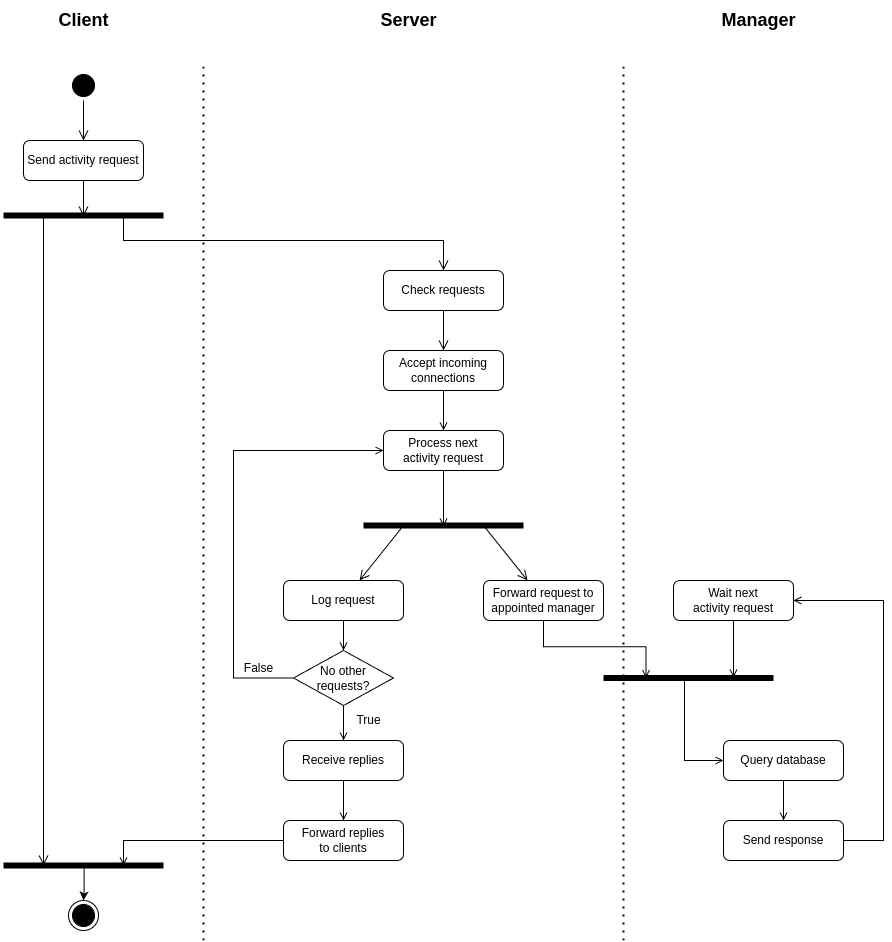
\includegraphics[scale=0.425]{images/Activity Diagram.png}
        
        \label{fig:activity_diagram}
    \end{figure}
    
    \subsection{State diagram}

    Come precedentemente accennato, ogni Manager in esecuzione su uno dei tre server corrisponde ad una macchina a stati finiti, la quale alterna tra uno stato di ricezione, stato di elaborazione e stato di invio della risposta. Tale comportamento risulta comune per tutti i Manager, senza alcuna azione aggiuntiva rispetto agli altri. 
    
    \begin{figure}[H]
        \centering
        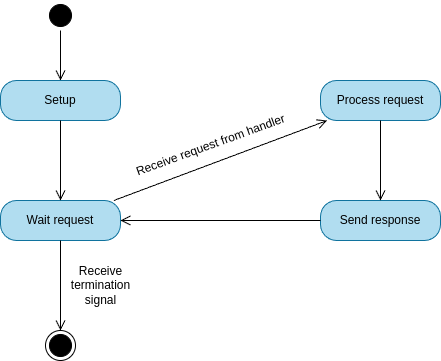
\includegraphics[scale=0.6]{images/Manager State Diagram.png}
        
        \label{fig:Manager_state_diagram}
    \end{figure}

    In particolare, è opportuno notare che ogni Manager rimanga in esecuzione permanente fino al momento in cui venga ricevuto un segnale di terminazione da parte del server. Una volta ricevuto tale segnale, ogni richiesta attualmente in elaborazione verrà scartata, senza comunicare alcun riscontro all'Handler associato.

    \newpage
    
    Analogamente, ognuno dei tre server può essere descritto come una macchina a stati finiti. Tuttavia, a differenza dei Manager, ogni server non rimarrà in attesa di una richiesta da parte di un client (dunque non si tratta di un'attesa bloccante). Bensì, nel caso in cui non vi sia alcuna richiesta entrante, il server procederà direttamente con la fase di controllo per eventuali risposte ricevute da parte dei Manager ad esso associati.
    
    \begin{figure}[H]
        \centering
        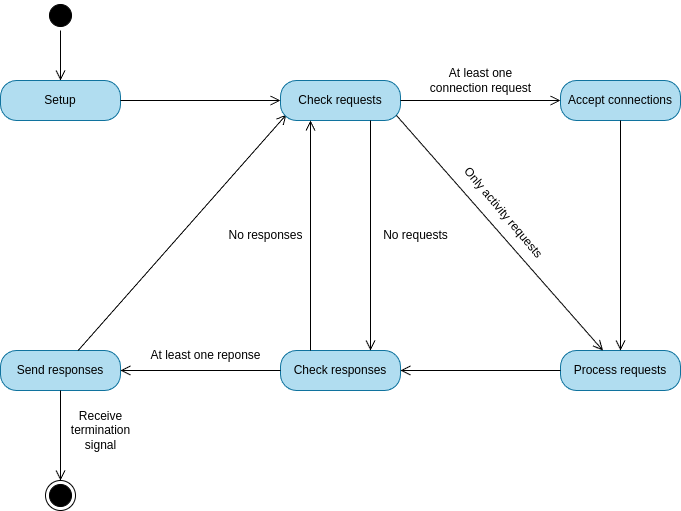
\includegraphics[scale=0.55]{images/Handler State Diagram.png}
        
        \label{fig:Handler_state_diagram}
    \end{figure}

    \newpage
    
    \subsection{Message sequence chart}
    
    Di seguito viene riportato il message sequence chart relativo all'invio di una richiesta da parte di un client, l'elaborazione di essa e dell'invio della risposta da parte del server. Tale processo risulta comune per tutti i server e i loro Manager, indipendentemente dal tipo di richiesta effettuata dal client. Inoltre, è necessario specificare che, nello scenario descritto, il client abbia già precedentemente stabilito la connessione con il server e che il Manager incaricato sia già attivo e pronto a ricevere e processare una richiesta.
    
    \begin{figure}[H]
        \centering
        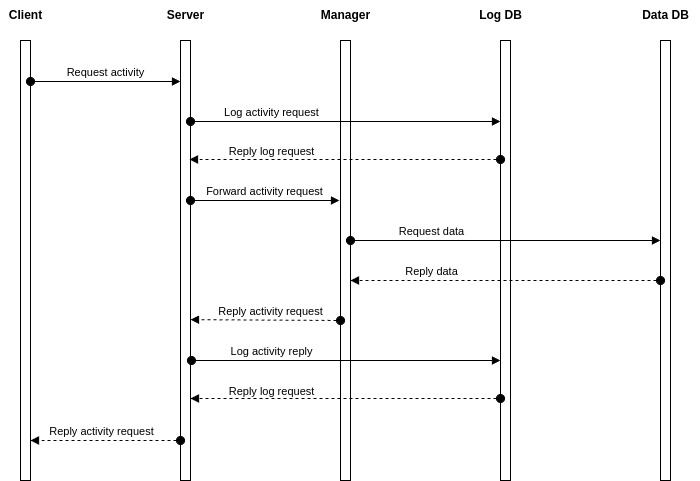
\includegraphics[scale=0.55]{images/Message Sequence Chart.png}
        
        \label{fig:message_sequence_chart}
    \end{figure}


    \chapter{Implementazione del software}
    
    \section{Struttura del codice}

    Trattandosi di tre server distinti, il codice è stato suddiviso in tre sezioni: una sezione \texttt{customer}, una sezione \texttt{courier} ed una sezione \texttt{supplier}. Ciascuna delle tre sezioni contiene al suo interno il codice relativo al proprio handler e i propri manager.

    Tuttavia, grazie alla suddivisione modulare tra server e handler, ognuno dei tre server è stato implementato tramite un'unica classe \texttt{Server}. Tale classe si interfaccia con i client esterni e con il sotto-modulo handler ad esso associato.
    
    Ciascuno degli handler possiede al suo interno una lista di richieste gestibili, ciascuna corrispondente ad un manager associato al server. Se ad un server viene inviata una richiesta non prevista dal proprio handler viene restituito un messaggio di "Bad Request". Inoltre, tutte le richieste e risposte passanti per un handler vengono loggate all'interno del DB dei log.

    A differenza dei server e gli handler, ciascun manager è stato implementato tramite un proprio file. Tale scelta deriva dalla differente conformazione dei manager all'interno delle attività da loro svolti: sebbene ciascuno di essi rispetti il modello di macchina a stati mostrato nelle sezioni precedenti, le operazioni previste da ogni stato cambiano leggermente tra un manager e l'altro, impedendo una generalizzazione completa tramite una singola classe. 

    \newpage

    Di seguito, vengono riportati gli pseudo-codici dei processi server e manager, incluso il sotto-modulo handler.
    
    \begin{verbatim}
Process Manager():
    connectToDB();
    connectToRedis();

    repeat untill sigterm is received:

        request = waitForRequest();

        If request is not valid:
            send("bad request");
        else:
            query = convertRequest();
            result = queryDB(query);

            If result is not valid:
                send("bad request");
            else:
                response = formatResponse(result)
                send(response);
                
Process Server():
    setupHandler();
    
    repeat until sigterm is received:

        requests = checkRequests();
        acceptIncomingConnections();
        
        if there are requests:
            foreach activity request:
                logRequest(request);
                isValidRequest = sendRequestToHandler(request);
               
                if not isValidRequest: 
                    sendToClient("bad request");

        responses = checkResponses();

        if there are responses:
            foreach response:
                sendToClient(response);
                
Component Handler():
    request = receiveRequestFromServer();
    request_type getRequestType();

    if request_type is not valid:
        return false
    else:
        sendToAppointedManager(request);
        return true
    \end{verbatim}
    

    \section{Struttura delle connessioni Redis}

    Ogni Handler istanzia 2 stream Redis per ogni Manager che controlla; ad esempio, per il Manager \texttt{Customer Sign Up} -- il quale prende il nome di \texttt{add-customer} all'interno del programma -- il \texttt{Customer Request Handler} istanzia uno stream per la comunicazione \textit{dall'Handler verso il manger}, ed un altro \textit{dal Manager verso l'Handler}.

    Al fine di tenere traccia dei vari customer che si interfacciano con il sistema, al momento della connessione il server assegna un ID ad ogni client, e tali ID vengono come prima chiave di ogni messaggio scambiato tra Handlers e Managers, permettendo agli Handlers di sapere a chi inoltrare la risposta.

    \newpage
    
    \section{Schema del database}
    
    \begin{figure}[H]
        \centering
        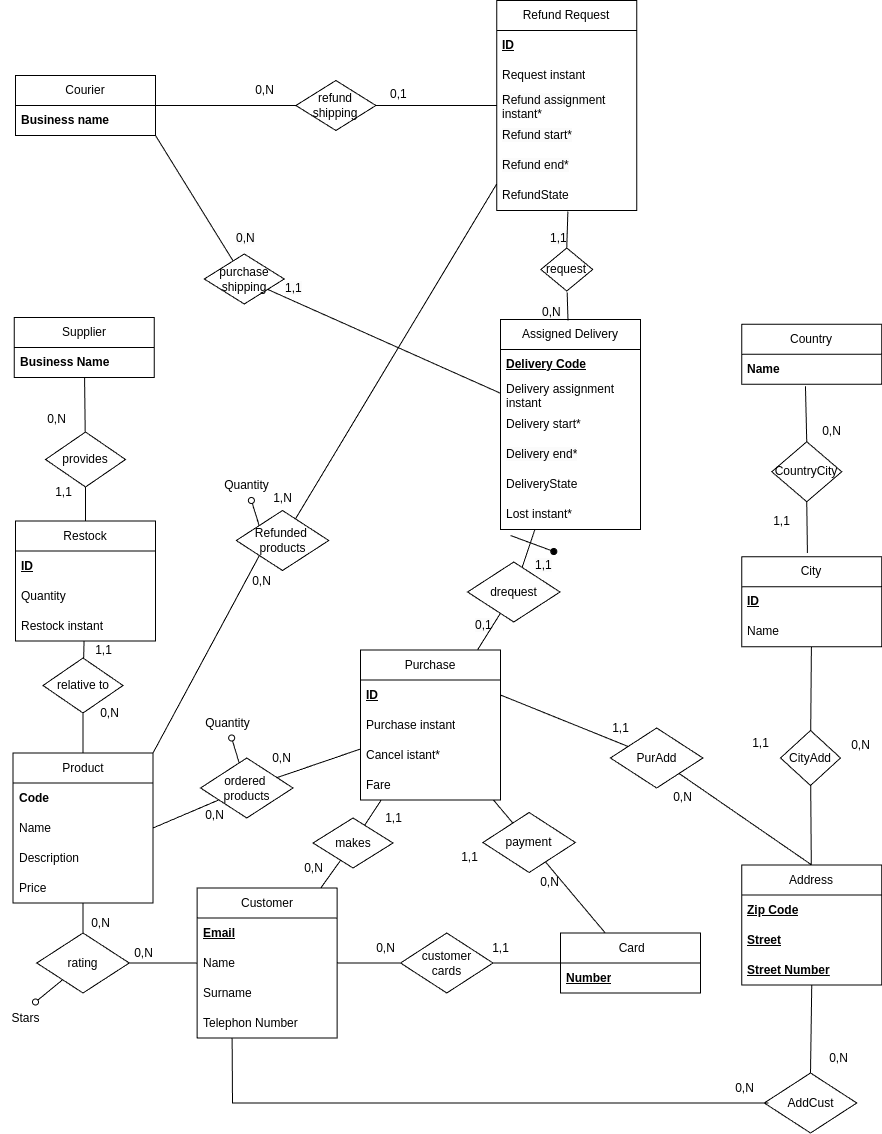
\includegraphics[scale=0.45]{images/ER-Restructured.png}
        
        \label{fig:message_sequence_chart}
    \end{figure}

    \newpage
    
    \section{Monitor funzionali}

    All'interno del software sono stati inseriti dei \textbf{monitor funzionali}, implementati tramite dei \textbf{trigger} all'interno del database dei dati. Tali trigger fungono da monitor attivi, impenendo che i dati all'interno del database siano inconsistenti tra loro o che non rispettino i vincoli esterni definiti nelle sezioni precedenti.

    Ad esempio, sono stati implementati i seguenti tre trigger:

    \begin{itemize}
    \item Trigger per la consistenza tra prodotti recensiti dall'utente e prodotti acquistati da esso

    \begin{verbatim}
    -- [V.Customer.ratingProdottiAcquistati]
    CREATE OR REPLACE FUNCTION consistent_rating()
    RETURNS TRIGGER AS $$
    BEGIN
        IF EXISTS (
            SELECT 1 FROM Customer, Product
            WHERE NEW.product = Product.code
            AND Customer.email = NEW.customer
            AND EXISTS (
                SELECT 1 FROM OrderedProducts, Purchase
                WHERE NEW.product = OrderedProducts.product
                AND Purchase.customer = Customer.email
                AND Purchase.id = OrderedProducts.purchase
            )
        ) IS FALSE THEN
            RAISE EXCEPTION 'invalid rating';
        END IF;
    
        RETURN NEW;
    END;
    $$ LANGUAGE plpgsql;
    
    CREATE TRIGGER consistent_rating_trg
    AFTER INSERT ON rating FOR EACH ROW
    EXECUTE FUNCTION consistent_rating();
    \end{verbatim}

    \item Trigger per la consistenza tra prodotti totali ordinati e prodotti presenti nello stock del fornitore

    \begin{verbatim}
    -- [V.Purchase.restockDisponibile]
    CREATE OR REPLACE FUNCTION ordered_product_quantity_consistency()
    RETURNS TRIGGER AS $$
    BEGIN
        IF (
            WITH restock_quantity AS (
                SELECT SUM(quantity) AS quantity
                FROM Restock
                WHERE product = NEW.product
            )
            SELECT SUM(DISTINCT rq.quantity) >= SUM(op.quantity)
            FROM OrderedProducts AS op, restock_quantity as rq
            WHERE op.product = NEW.product
        ) IS FALSE THEN
            RAISE EXCEPTION 'invalid quantity for order request';
        END IF;
    
        RETURN NEW;
    END;
    $$ LANGUAGE plpgsql;
    
    CREATE TRIGGER ordered_product_quantity_consistency_trg
    AFTER INSERT ON OrderedProducts FOR EACH ROW
    EXECUTE FUNCTION ordered_product_quantity_consistency();
    \end{verbatim}

    \newpage
    
    \item Trigger per la consistenza tra prodotti rimborsati e prodotti acquistati dall'utente

    \begin{verbatim}
-- [V.RefoundRequest.prodottiConsistenti]
CREATE OR REPLACE FUNCTION refunded_products_consistency()
RETURNS TRIGGER AS $$
BEGIN
    IF EXISTS (
        SELECT 1 
        FROM RefundRequest AS rr, AssignedDelivery AS ad,
        Purchase AS p, OrderedProducts as op
        WHERE NEW.refund_request = rr.id 
        AND rr.assigned_delivery = ad.delivery_code
        AND ad.purchase = p.id
        AND op.purchase = p.id
        AND op.product = NEW.product
    ) IS FALSE THEN
        RAISE EXCEPTION 'invalid refund request';
    END IF;

    RETURN NEW;
END;
$$ LANGUAGE plpgsql;

CREATE TRIGGER refunded_products_consistency_trg
AFTER INSERT ON RefundedProduct FOR EACH ROW
EXECUTE FUNCTION refunded_products_consistency();
    \end{verbatim}
        
    \end{itemize}

    \underline{\textbf{Nota}}: ulteriori trigger funzionali possono essere trovati all'interno del file \texttt{db-scripts/triggers.sql}.

    \newpage
    
    \section{Monitor non-funzionali}

\begin{verbatim}

while(true) {
    query = "
        SELECT EXTRACT(
            EPOCH FROM AVG(disconnection_instant - connection_instant)
        ) * 1000 as avg
        FROM Client
        WHERE disconnection_instant IS NOT NULL
    ";

    average = log_db.execQuery(query);

    if average <= MAX_CONNECTION_TIME_AVG:
        responseStatus = "SUCCESS";
    else:
        responseStatus = "ERROR";

    query = "
        INSERT INTO
        SessionStatistic(type, end_instant, value, response_status)
        VALUES ('Session', CURRENT_TIMESTAMP, average, responseStatus)
    ";

    log_db.execQuery(query);

    query = "
        SELECT EXTRACT(
            EPOCH FROM AVG(response_instant - request_instant)
        ) * 1000 as avg
        FROM Communication
        WHERE response_instant IS NOT NULL
    ";

    average = log_db.checkQueryResult(query);

    
    if average <= MAX_RESPONSE_TIME_AVG:
        responseStatus = "SUCCESS";
    else:
        responseStatus = "ERROR";

    query = "
        INSERT INTO
        SessionStatistic(type, end_instant, value, response_status)
        VALUES ('Response', CURRENT_TIMESTAMP, average, responseStatus)
    ";

    log_db.execQuery(query);

    sleep(60sec);
}

\end{verbatim}

\quad

    \section{Risultati sperimentali}

    Nel suo intero, il sistema rappresenta una piattaforma e-commerce consona agli standard moderni e può essere effettivamente utilizzato tramite le API documentate all'interno del file \texttt{README.md} associato con questa cartella.

    I risultati riscontrati tramite il test generator mostrano che la piattaforma sia in grado di gestire correttamente eventuali sovraccarichi tramite la parallelizzazione delle richieste ed eventuali input erronei o inconsistenti.
\end{document}